\subsection{Infrasegmental Government (IG)}

\textquote[{\cite[p.~64]{scheer2004}}]{%
  (49) Infrasegmental Government (IG) - final version
  \begin{enumerate}
  \item a consonant A may contract a governing relation
    with its neighbour iff there is a place-defining
    autosegmental line where A possesses a prime,
    while the corresponding slot in the internal
    structure of B is empty.
    In this situation, the prime belonging to A governs
    the empty position of B.
  \item the empty Nucleus that is enclosed within such
    a domain of Infrasegmental Government is circumscribed.
    Its Empty Category Principle is satisfied.  
  \end{enumerate}
  Infrasegmental Government is the equivalent of
  Proper Government at the level of the internal
  structure of segments.
  At the syllabic level, Proper Government describes
  a lateral relation whereby a contentful position
  establishes Government over an empty position.
  Infrasegmental Government does the same thing
  below the skeleton
  (and is therefore called "infrasegmental").%
}

\textquote[{\cite[p.~65]{scheer2004}}]{%
  \begin{definition}[50]\textbf{Government Licensing}
    
    a domain of Infrasegmental Government may only be
    established if the head of the domain is licensed to
    act as a governor by its own Nucleus.
    Only contentful Nuclei are able to license.
  \end{definition}
  
  The notion of Government Licensing has been introduced by
  Charette (1990,1991) in a different syllabic environment,
  and using different vocabulary.\textsuperscript{38}
  The very idea expressed by Government Licensing, however,
  is independent from any particular syllabic theory.
  It expresses a fundamental insight into the relationship
  between consonants and vowels in phonology:
  consonant clusters need a vocalic support
  in order to exist.
  
  In CVCV, the licensing condition on Infrasegmental
  Government has the effect of excluding consonantal
  clusters before empty Nuclei.
  This is shown under (51) below.%
}

\subsubsection{Internal structure of consonants}

4 primes define place of articulation:
I (palatality), U (velarity), A (aperture) and B (labiality/roundness)
\cite[p.~63]{scheer2004}

\textquote[{\cite[p.~6]{scheer2012}}]{\small
  For there are other areas in phonology where arboreal structure is
  traditionally assumed: below the skeleton for the representation of
  melody (Feature Geometry), above the skeleton for the representation
  of morpho-syntactic information (the Prosodic Hierarchy).
  While unary melodic representations (Anderson \& Jones 1974 and ensuing
  applications in Dependency Phonology, Particle Phonology and
  Government Phonology) provide a non-arboreal alternative for the former%
}

\paragraph{A (aperture)}
\begin{itemize}
\item nasals \cite[p.~55]{scheer2004}
\item \textquote[{\cite[p.~53]{scheer2004}}]{%
  The prime A co-defines the consonantal identities of the labio-dental and
  the palatoalveolar locus, but is absent from bilabial segments}
\end{itemize}

\paragraph{U (velarity)}
\textipa{[r,l,n]} \cite[p.~55]{scheer2004}

\paragraph{I (palatality)}
\textipa{[\c{c}]} (palatalisation of \textipa{[X]})
  \begin{itemize}
  \item genau dann wenn nach Segment mit I
  \item coronale sonoranten \textipa{[n,l,r]} = I-provider
  \end{itemize}
  \cite[p.~56]{scheer2004}

\paragraph{? (occlusion)}

\paragraph{}
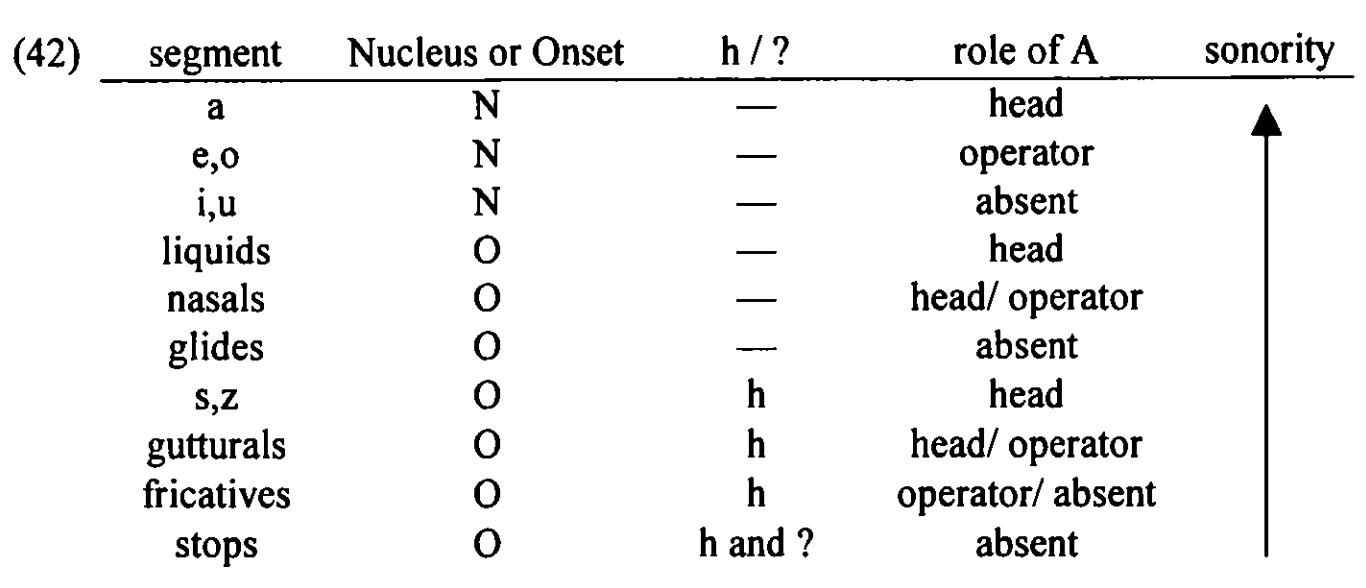
\includegraphics[width=.5\textwidth]{figures/phon-primes-ah-sonority.png}
\cite[p.~52]{scheer2004}

\paragraph{Interaction}
\begin{itemize}
\item \enquote{A and ? hate each other: they cannot compine}\cite[p.~52]{scheer2004}
\end{itemize}

\subsubsection{Lexicon}
\textquote[{\cite[p.~145]{scheer2012}}]{
  That is, there are no lateral relations left that are recorded in the
  lexicon -- except Infrasegmental Government, which defines a TR cluster
  as a branching onset in the lexicon (see Vol.1 §149 on the particular
  status of this device).
  Significantly, though, Infrasegmental Government operates below the
  skeleton and, unlike government and licensing,
  is sensitive to melodic properties.
  It may thus be safely concluded that it belongs to the melodic world [\emph]
}